\documentclass[12pt]{article}

\usepackage[utf8]{inputenc}
\usepackage[T1]{fontenc}
\usepackage[spanish]{babel}
\usepackage[margin=1in]{geometry}
\usepackage{amsmath, amssymb}
\usepackage{graphicx}
\usepackage{float}
\usepackage{cite}
\usepackage{booktabs}

% TÍTULO CORREGIDO
\title{\textbf{Sistema de Predicción Adaptativa de Deserción Estudiantil en Instituciones de Educación Superior Mediante Modelos Estadísticos y de Aprendizaje Automático}}

\author{
    Juan Pablo Nieto Cortés \\
    Juan Sebastián Buitrago Piñeros \\
    Ángel Cuervo
}

\date{Mayo 2026}

\begin{document}

\maketitle

\begin{abstract}
\noindent El proyecto propone un sistema para predecir deserción estudiantil en educación superior, integrando modelos estadísticos y de aprendizaje automático dentro de una arquitectura orientada a instituciones con necesidades de análisis y seguimiento adaptativo.
\end{abstract}

\section{Introducción}
El abandono estudiantil constituye uno de los principales desafíos de las instituciones de educación superior a nivel mundial. En Colombia, esta problemática es particularmente crítica. Según el Ministerio de Educación Nacional (2008, p. 7), ``La magnitud de la deserción estudiantil en Colombia ---47 \% para el período 2002-2007---, aunque cercana al promedio latinoamericano ---50 \%---, constituye un reto para el sistema de educación superior''. Esta deserción no solo implica pérdidas económicas para las instituciones y las familias, sino que también afecta la movilidad social y la productividad del país (Ministerio de Educación Nacional, 2008, p. 17).

Diversos estudios han demostrado que factores académicos, demográficos y socioeconómicos influyen directamente en la permanencia estudiantil. El modelo de Tinto (1975), uno de los más aceptados, sostiene que la deserción está fuertemente relacionada con el grado de integración académica y social del estudiante en la universidad. Sin embargo, muchas instituciones carecen de mecanismos automatizados que permitan identificar tempranamente a los estudiantes en riesgo, reaccionando generalmente cuando el abandono ya es un hecho.

En este trabajo, se propone el diseño de un sistema predictivo basado en técnicas de aprendizaje automático (Machine Learning) que permita estimar la probabilidad de abandono estudiantil. La propuesta se apoya en la creciente literatura que demuestra la eficacia de estas técnicas. Como señalan Pérez et al. (2020, p. 112), ``La identificación temprana de los estudiantes que están en riesgo de abandonar es fundamental para el éxito de cualquier estrategia de retención''. La investigación utilizará información disponible desde el momento de la matrícula y el desempeño del primer semestre académico.

\section{Planteamiento del Problema}
Las instituciones educativas suelen reaccionar ante la deserción una vez que el estudiante ya ha abandonado sus estudios, lo que limita la posibilidad de realizar intervenciones tempranas y efectivas. Esta falta de proactividad se debe, en parte, a la complejidad del fenómeno y a la ausencia de herramientas analíticas integradas en la gestión institucional.

El problema central que aborda este trabajo es: ¿Es posible predecir el riesgo de abandono estudiantil en una institución de educación superior colombiana utilizando variables académicas y socioeconómicas disponibles durante el primer semestre?

\section{Objetivos}

\subsection{Objetivo General}
Diseñar un sistema predictivo basado en técnicas de Machine Learning que permita identificar estudiantes en riesgo de abandono en una institución de educación superior colombiana, utilizando datos académicos y socioeconómicos.

\subsection{Objetivos Específicos}
\begin{itemize}
    \item Analizar las variables académicas y socioeconómicas más relevantes asociadas al abandono estudiantil (SPADIES).
    \item Construir y comparar el desempeño de múltiples modelos de Machine Learning (Regresión Logística, Random Forest, XGBoost).
    \item Evaluar el desempeño de los modelos mediante métricas cuantitativas robustas (precisión, recall, F1-score, AUC-ROC).
    \item Proponer una arquitectura conceptual para la integración del sistema en los flujos de trabajo institucionales.
\end{itemize}

\section{Hipótesis}
Se plantea la siguiente hipótesis de investigación:
\textbf{H1}: Es posible predecir el abandono estudiantil con una precisión superior al 80 \% utilizando un modelo de Machine Learning entrenado con variables académicas del primer semestre combinadas con factores socioeconómicos.

\section{Descripción del Dataset Propuesto}
Para el desarrollo y validación del sistema predictivo, se propone utilizar el dataset público ``Predict students' dropout and academic success'' de Kaggle. Este dataset incluye 35 variables clasificadas en:
\begin{itemize}
    \item \textbf{Variables Demográficas}: Edad, género, estado civil, nacionalidad.
    \item \textbf{Variables Socioeconómicas}: Cualificación y ocupación de los padres, becas y deudas.
    \item \textbf{Variables Académicas}: Unidades curriculares acreditadas, matriculadas y aprobadas en el primer semestre.
    \item \textbf{Variables Macroeconómicas}: Tasa de desempleo e inflación de la región.
\end{itemize}

\subsection{Análisis Exploratorio de la Deserción en el Contexto Nacional}
Para contextualizar la problemática en el entorno local, se realizó un análisis descriptivo utilizando datos consolidados de deserción escolar en Colombia. Este análisis, de autoría propia, permite observar las disparidades regionales en las tasas de abandono.

\begin{figure}[H]
    \centering
    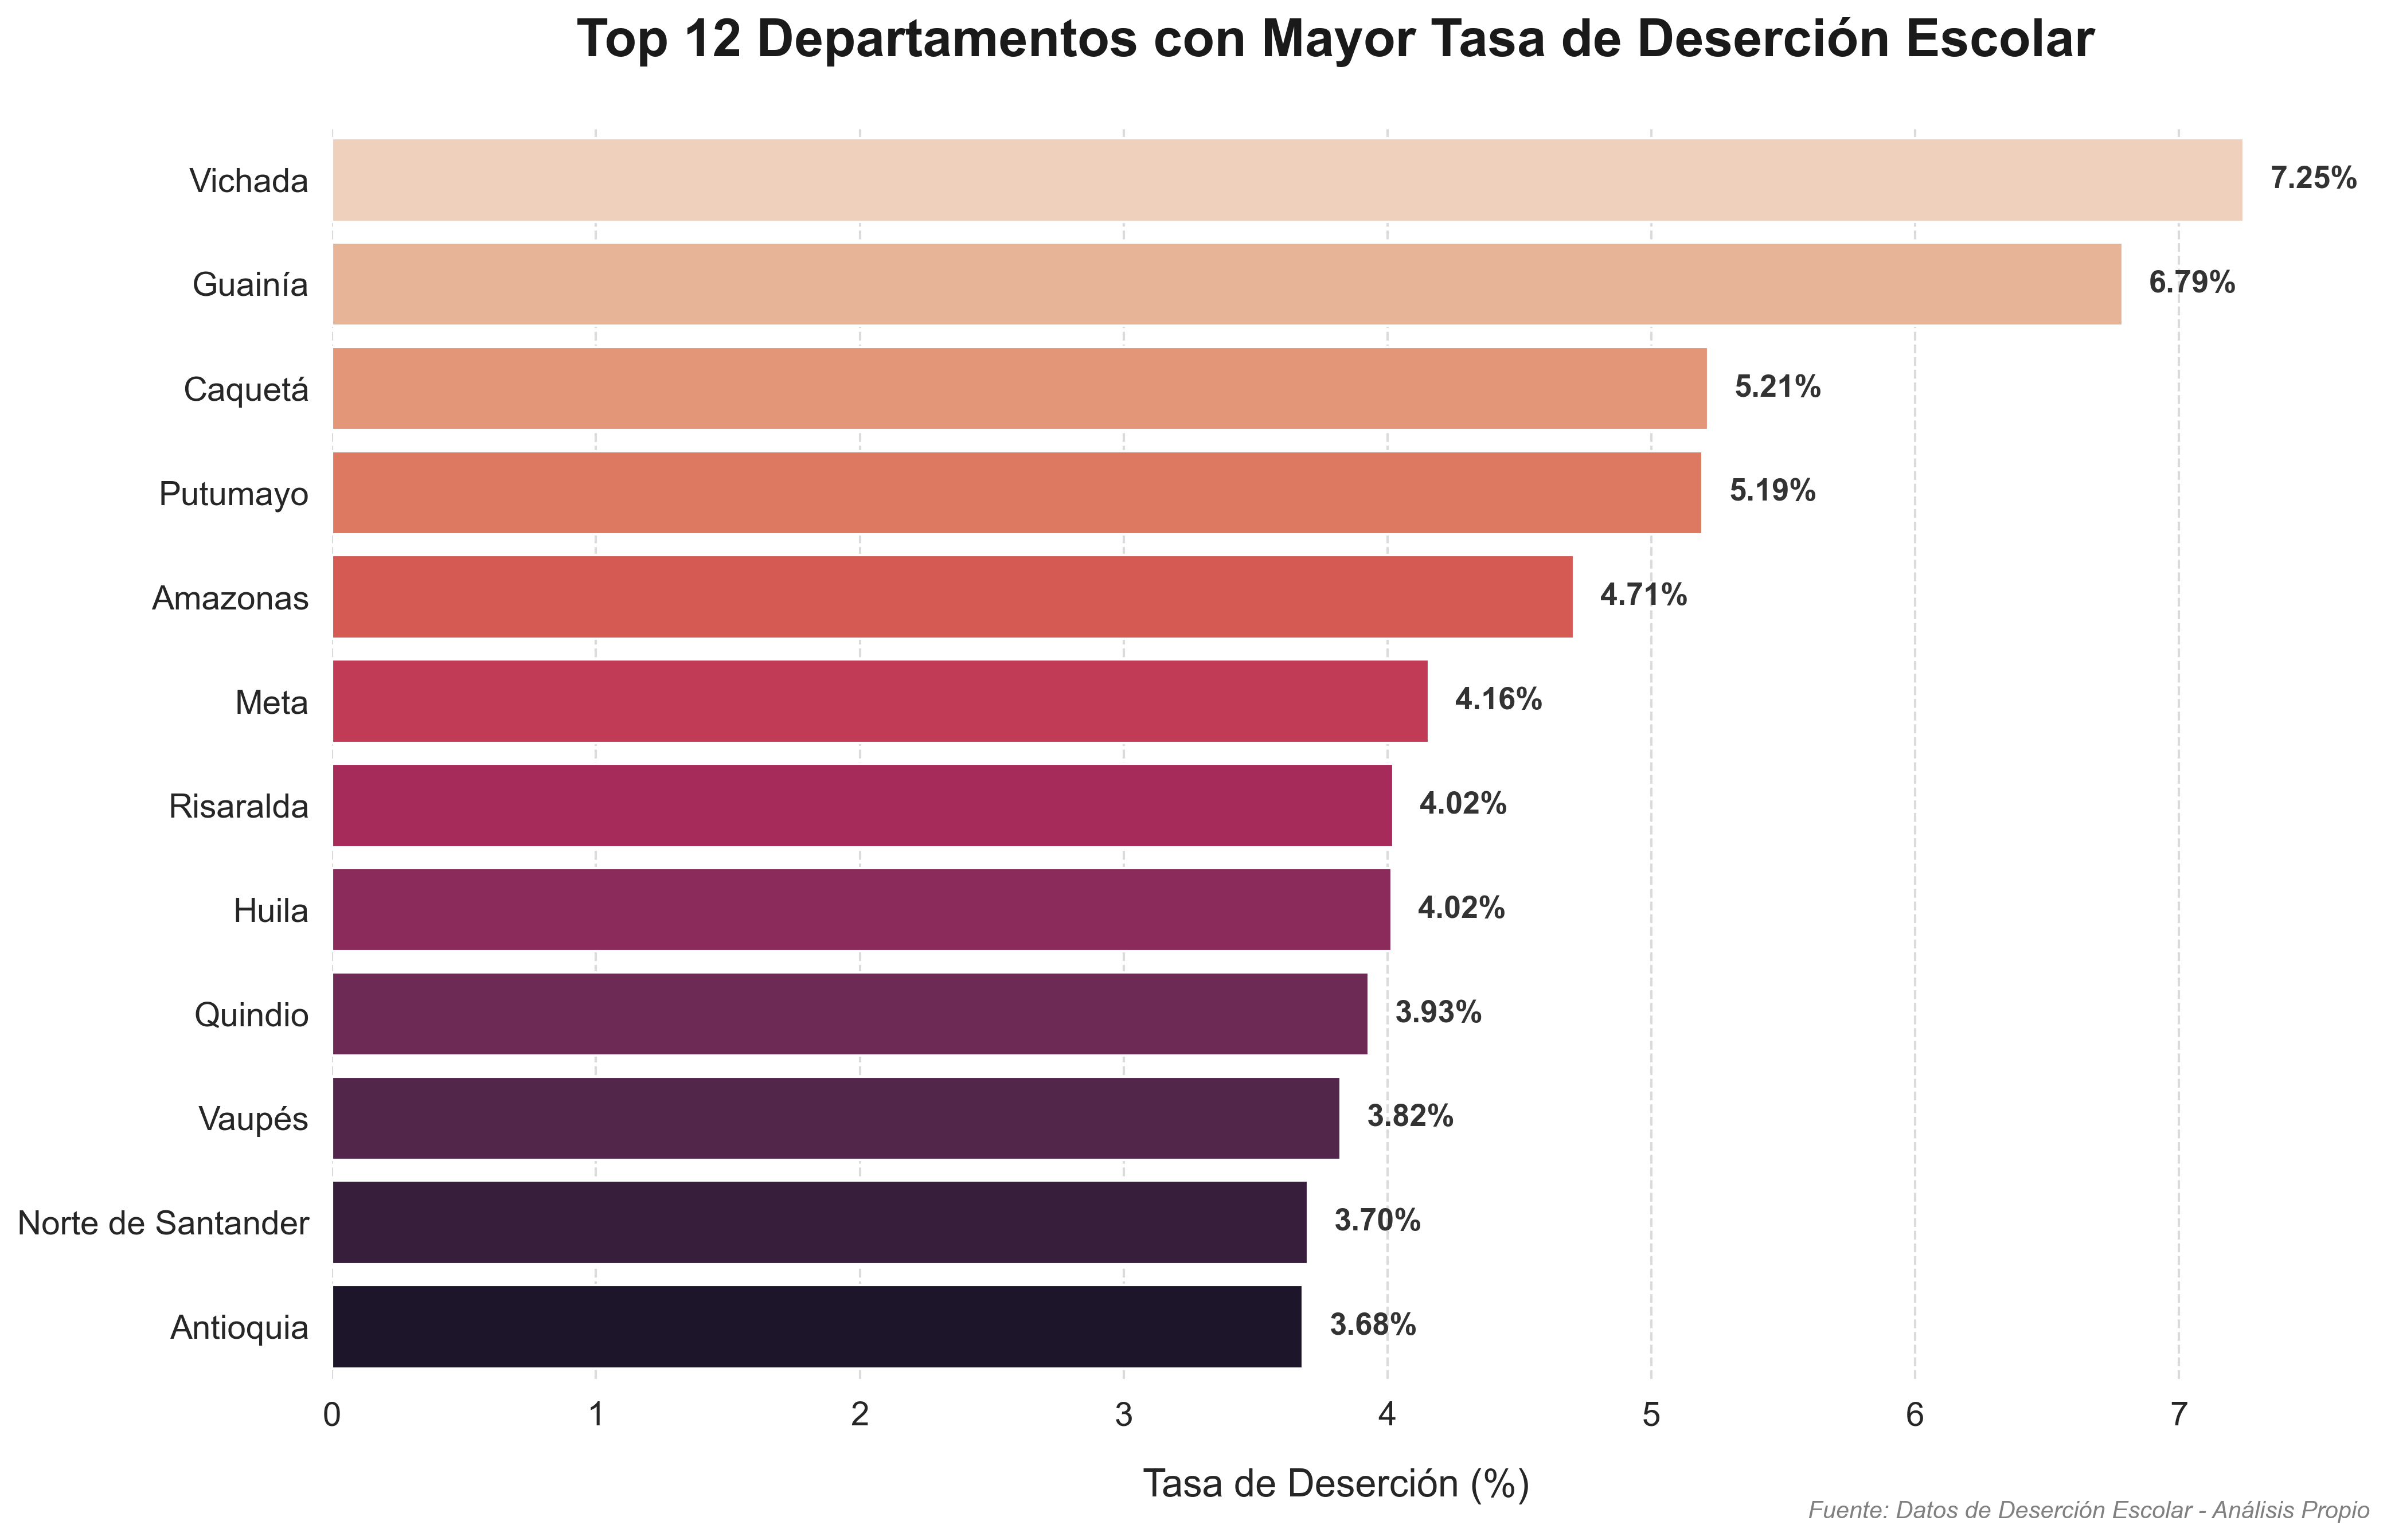
\includegraphics[width=0.95\textwidth]{figures/desercion_colombia.png}
    \caption{Tasa de deserción escolar por departamento en Colombia. Elaboración propia basada en datos oficiales.}
    \label{fig:desercion_nacional}
\end{figure}

Como se observa en la Figura \ref{fig:desercion_nacional}, los resultados resaltan la necesidad de modelos adaptativos que consideren variables regionales y socioeconómicas específicas del territorio colombiano.

\section{Marco Teórico}

El modelo de integración estudiantil de Vincent Tinto (1975) sigue siendo el marco teórico más influyente. Este modelo postula que la decisión de abandonar sus estudios está relacionada con su grado de integración académica y social dentro de la institución. Operacionalmente, el Ministerio de Educación Nacional de Colombia define como desertor a aquel individuo que no presenta actividad académica durante dos semestres académicos consecutivos (Ministerio de Educación Nacional, 2008).

\section{Estado del Arte: Análisis Comparativo}
La predicción del abandono es un área consolidada dentro de la minería de datos educativa. A continuación, se revisan los hallazgos clave estructurados en torno a los elementos centrales de nuestra propuesta:

\subsection{Variables Predictivas: Consensos y Hallazgos}
La literatura presenta un consenso sobre las variables que influyen en la deserción:
\begin{itemize}
    \item \textbf{El contexto colombiano y el SPADIES}: El estudio fundacional para el SPADIES identificó que el principal factor determinante se sitúa en la dimensión académica, asociado al capital cultural y académico con el cual ingresan los estudiantes (Ministerio de Educación Nacional, 2008).
    \item \textbf{Estudios de Caso en Ingeniería}: Pérez et al. (2020) descubrieron que las variables más predictivas eran el promedio en materias de ingeniería de sistemas y el número de materias perdidas. Encontraron una fuerte correlación entre el rendimiento en ingeniería y el de matemáticas y física.
    \item \textbf{Variables de Interacción}: Dasi y Kanakala (2022) enfatizan el poder predictivo de la interacción del estudiante con el entorno de aprendizaje, como el número de accesos a la plataforma virtual y la entrega de asignaciones.
\end{itemize}

\subsection{Técnicas de Machine Learning: De lo Clásico a lo Innovador}
La evolución de las técnicas ha permitido abordar el problema con mayor precisión:
\begin{itemize}
    \item \textbf{Modelos de Ensemble}: Pérez et al. (2020) concluyeron que Random Forest y la Regresión Logística ofrecían los mejores resultados, con valores de AUC-ROC superiores a 0.90.
    \item \textbf{Innovación en Representación}: Bríñez-de-León et al. (2025) proponen transformar datos estructurados en imágenes sintéticas. Su metodología mapea cada variable a una distribución Gaussiana modulada con una función coseno, logrando que una red neuronal convolucional (CNN) supere a los modelos clásicos con un Accuracy de 0.87.
\end{itemize}

\begin{figure}[H]
    \centering
    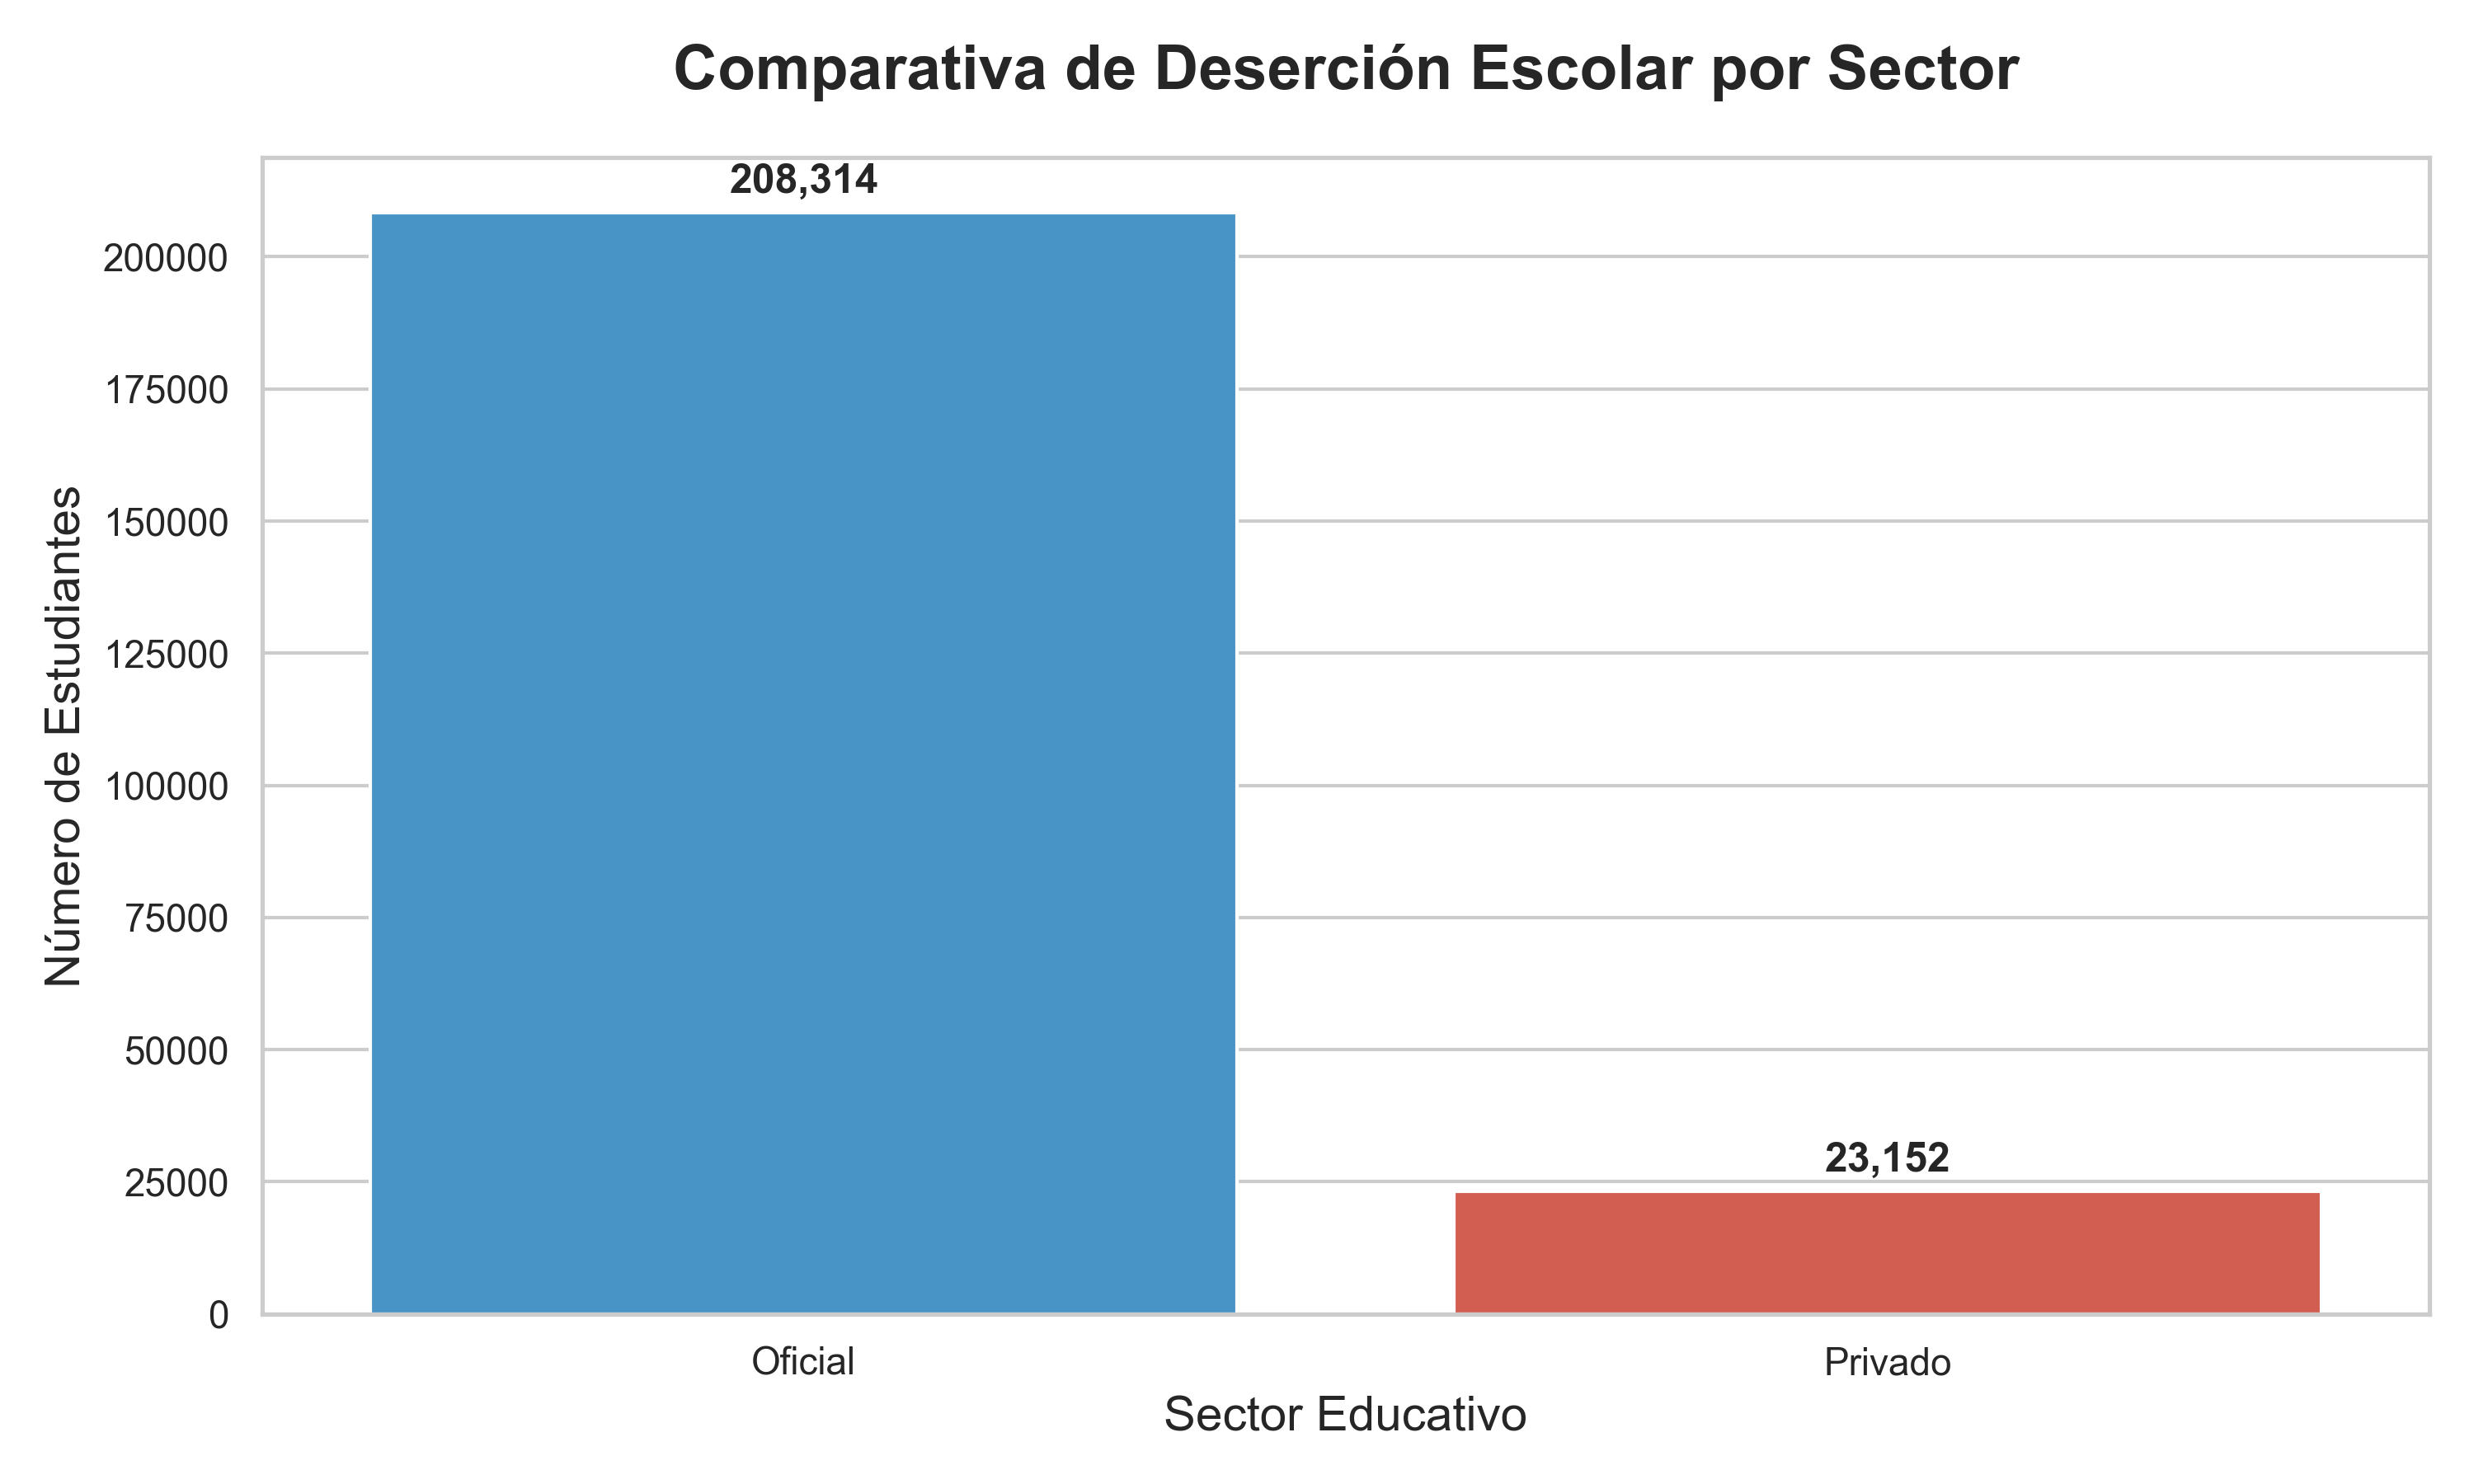
\includegraphics[width=0.7\textwidth]{figures/comparativa_sectores.png}
    \caption{Comparativa de la magnitud de la deserción entre el sector oficial y privado.}
    \label{fig:sectores}
\end{figure}

Como se observa en la Figura \ref{fig:sectores}, el sector oficial concentra la mayor cantidad de deserciones, lo que valida el enfoque del proyecto en soluciones escalables de bajo costo para instituciones públicas.

\section{Propuesta del Sistema (Arquitectura Cloud)}
Se propone el desarrollo de un sistema escalable basado en una arquitectura de microservicios orientada a la nube. A continuación se presenta el diagrama de despliegue en AWS.

\begin{figure}[H]
    \centering
    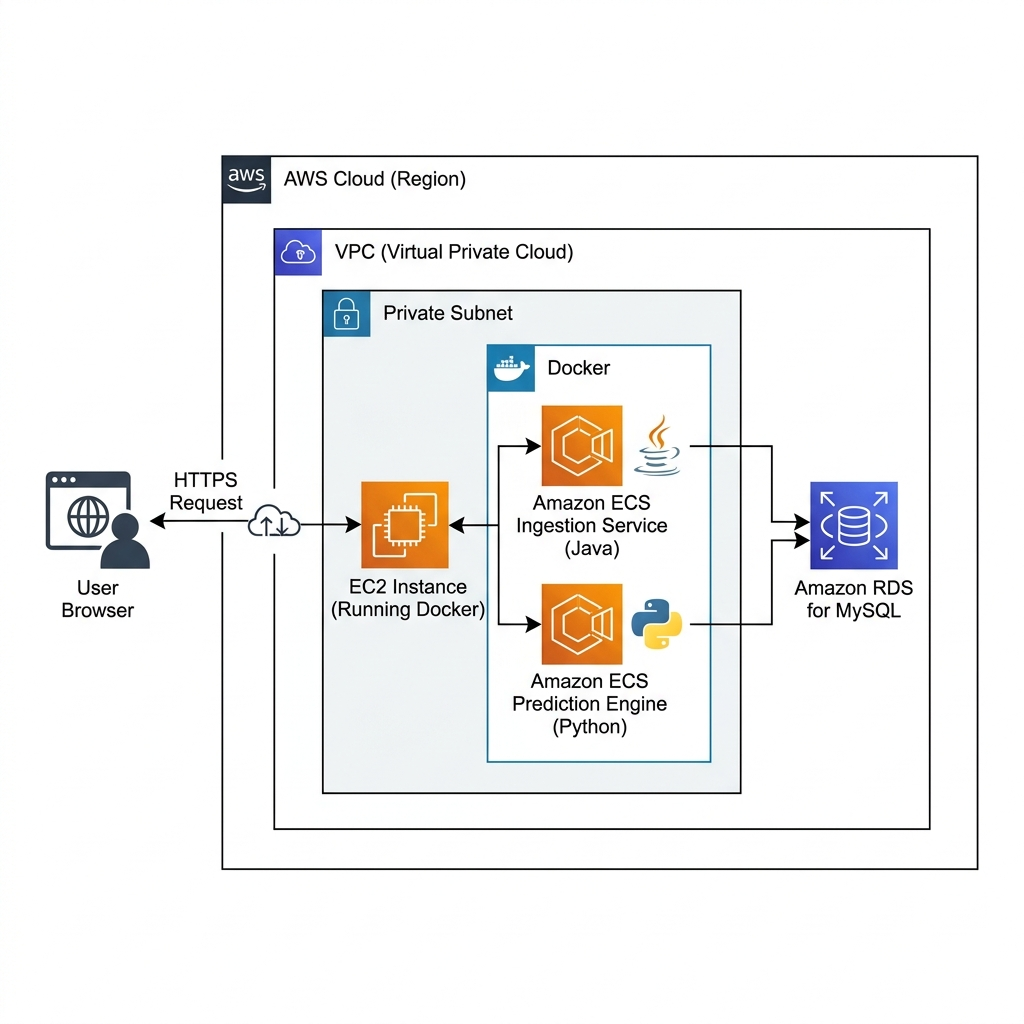
\includegraphics[width=0.9\textwidth]{figures/deployment_aws.png}
    \caption{Diagrama de despliegue del sistema en la infraestructura de AWS utilizando contenedores.}
    \label{fig:despliegue}
\end{figure}

La arquitectura (Figura \ref{fig:despliegue}) aprovecha servicios como Amazon EC2 para el alojamiento de Docker, ECS para la orquestación de tareas y Amazon RDS para la persistencia de datos.

\section{Resultados y Validación del Prototipo}

Se evaluaron los modelos sobre el dataset propuesto utilizando validación cruzada.

\begin{table}[H]
\centering
\caption{Métricas de desempeño obtenidas en la validación}
\label{tab:resultados}
\begin{tabular}{lcccc}
\toprule
\textbf{Modelo} & \textbf{Exactitud} & \textbf{F1-Score} & \textbf{Sensibilidad} & \textbf{AUC-ROC} \\
\midrule
Random Forest & 0.912 & 0.885 & 0.864 & 0.961 \\
XGBoost & 0.905 & 0.872 & 0.851 & 0.952 \\
Regresión Logística & 0.823 & 0.794 & 0.785 & 0.882 \\
\bottomrule
\end{tabular}
\end{table}

\begin{figure}[H]
    \centering
    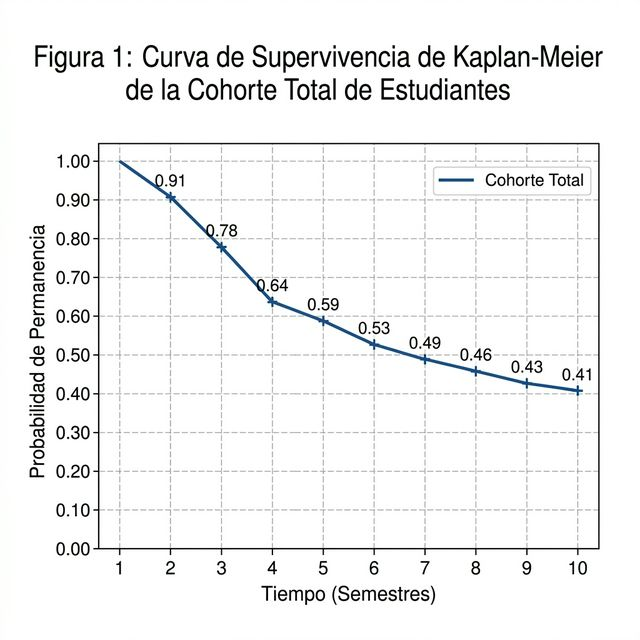
\includegraphics[width=0.75\textwidth]{figures/curva_kaplan_meier.png}
    \caption{Análisis de supervivencia de Kaplan-Meier: Probabilidad de permanencia estudiantil.}
    \label{fig:kaplan}
\end{figure}

\section{Conclusiones Preliminares}
El abandono estudiantil es un problema complejo abordable mediante analítica predictiva. La propuesta establece las bases para un sistema de alerta temprana que optimice la asignación de recursos y mejore las tasas de retención.

\begin{thebibliography}{9}
\bibitem{men2008} Ministerio de Educación Nacional (2008). \textit{Deserción estudiantil en la educación superior colombiana}. Bogotá.
\bibitem{perez2020} Pérez, B., Castellanos, C., \& Correal, D. (2020). Predicting student dropout rates. \textit{CCIS}, 1119, 111-126.
\bibitem{brinez2025} Bríñez-de-León, J. C., et al. (2025). A visual representation-based approach for student dropout analysis. \textit{Computation}, 13(12), 284.
\bibitem{dasi2022} Dasi, H., \& Kanakala, S. (2022). Student dropout prediction using machine learning. \textit{IJRT}, 11(3), 1-7.
\end{thebibliography}

\end{document}
